\section{Proposed Method}
\label{sec:method}

The proposed framework embeds the MDP state using a
GNN~\cite{gilmer2017neural}, and decides fire or hold for every weapon. The
greedy marginal-value rule assigns targets to the firing
weapons. A fixed local search then revises the completed schedule. Only the
fire-or-hold decision is learned. Fig.~\ref{fig:overall} shows the pipeline
and Algorithm~\ref{alg:scope} states it precisely.

%% Figure generated by paper/make_overall_figure.py (matplotlib). Edit that
%% script and re-run it rather than editing the PNG. Grayscale by design.
\begin{figure}[htbp]
  \centering
  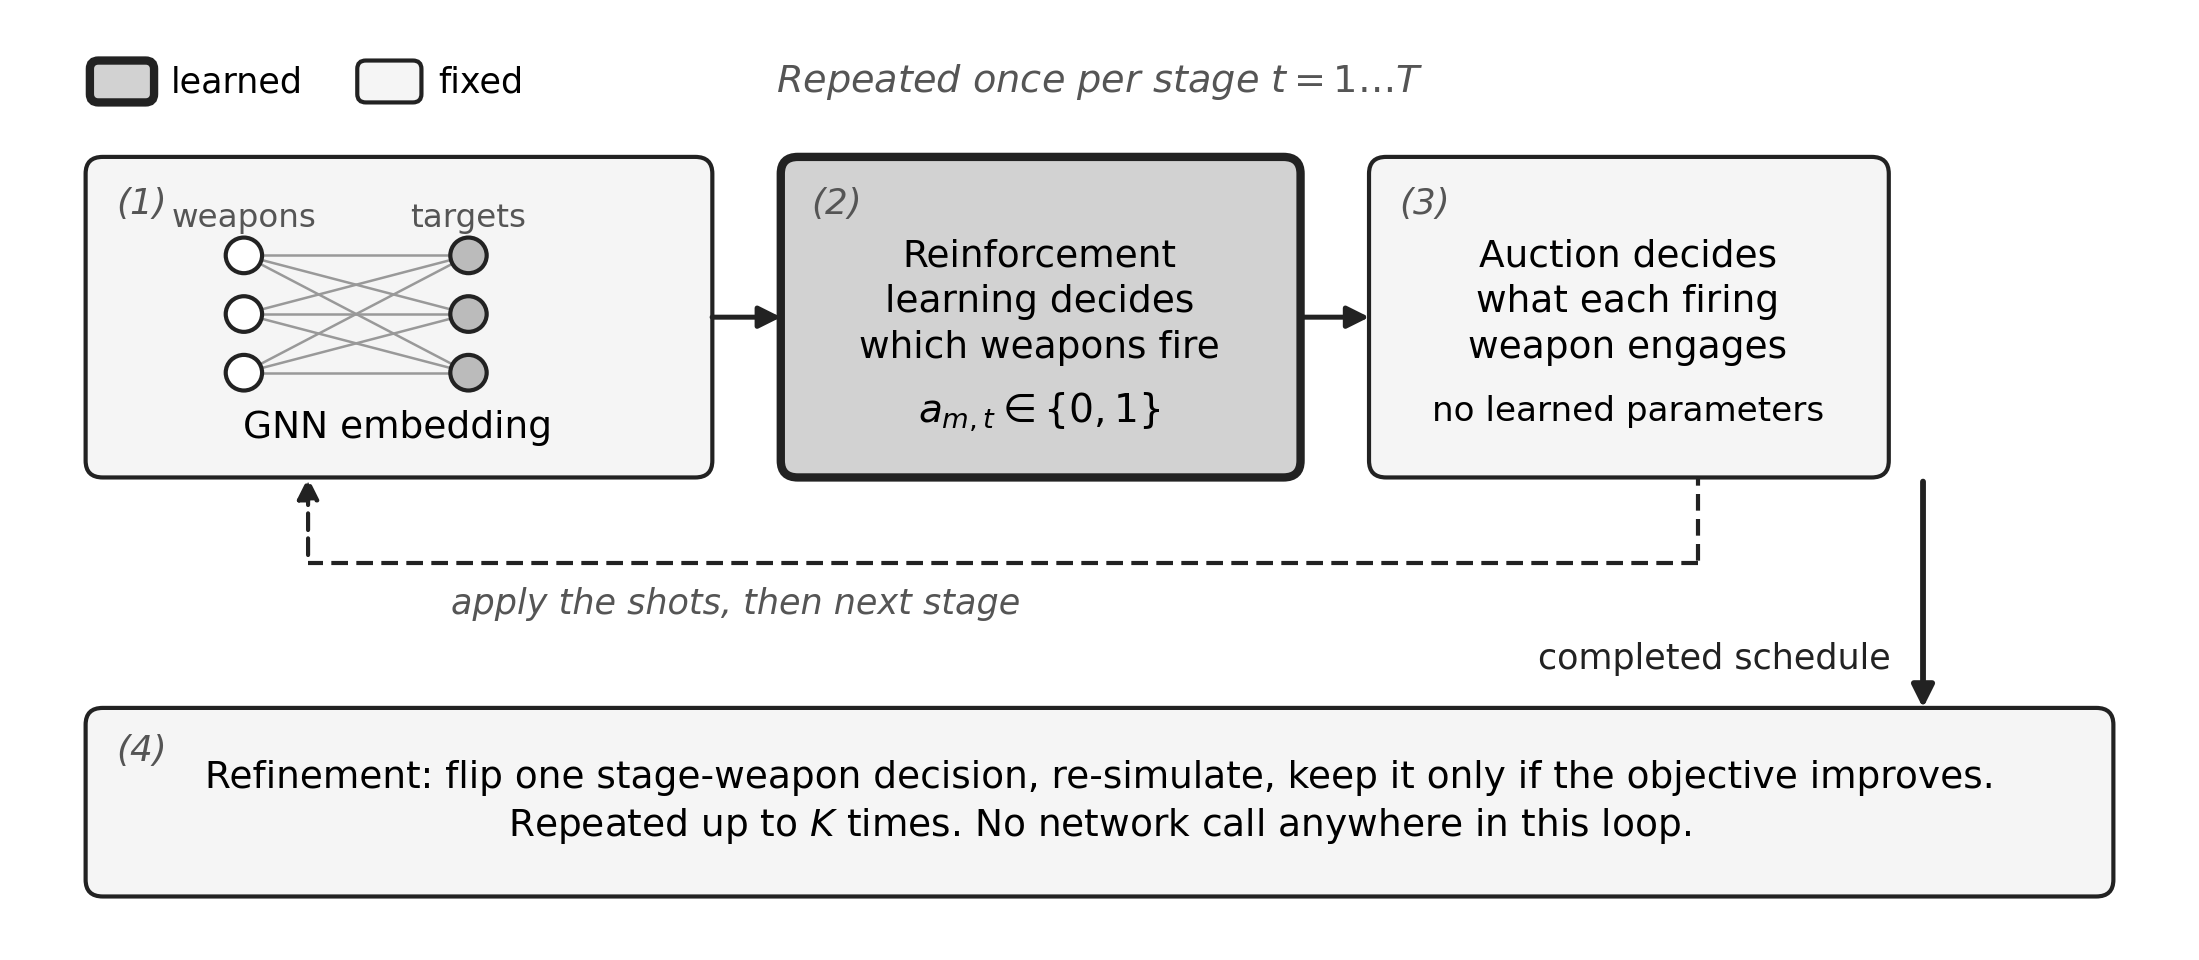
\includegraphics[width=\columnwidth]{figure/Overall.png}
  \caption{The pipeline, corresponding step for step to
  Algorithm~\ref{alg:scope}. Border weight marks the one learned box: the
  policy emits one bit per weapon and nothing else.}
  \label{fig:overall}
\end{figure}

\begin{algorithm}[htbp]
\caption{Inference: construction followed by fixed local search}
\label{alg:scope}
\begin{algorithmic}[1]
\Require instance $(V, P, A, D, TW)$; participation policy $\pi_\theta$; edit budget $K$
\Ensure feasible schedule
\Statex \textbf{Construction}
\State $s_1 \gets$ initial state
\For{$t = 1$ \textbf{to} $T$}
  \State $H^{\text{wpn}}, H^{\text{tgt}}, H^{\text{edge}} \gets \textsc{Encode}(s_t)$ \Comment{$L$ message-passing rounds, Sec.~\ref{sec:encoding}}
  \State $a_{m,t} \gets \mathbb{1}\!\left[\pi_m(\text{fire}\mid s_t) > \tfrac12\right]$ for all $m$ \Comment{one forward pass, Eq.~\eqref{eq:fire-prob}}
  \State $F_t \gets \{m : a_{m,t} = 1\}$
  \State $x_t \gets \textsc{Assign}(F_t, s_t)$ \Comment{many-to-one, Sec.~\ref{sec:auction}}
  \State $s_{t+1} \gets \textsc{Step}(s_t, x_t)$
\EndFor
\State $\phi \gets \bm{0}$; \; $\mathit{tried} \gets \emptyset$; \; $J^\star \gets J(\phi)$
\Statex \textbf{Fixed local search (Sec.~\ref{sec:local-search})}
\For{$k = 1$ \textbf{to} $K$}
  \If{$\mathit{tried}$ covers every slot} \textbf{break} \Comment{1-flip local optimum} \EndIf
  \State draw $(t^\ast\!, m^\ast)$ uniformly from the untried slots
  \State $\phi' \gets \phi$ with $\phi'_{t^\ast\!,m^\ast}$ flipped
  \State $J' \gets J(\phi')$ \Comment{re-simulate: assignment + environment only, no network call}
  \If{$J' < J^\star$}
    \State $\phi \gets \phi'$; \; $J^\star \gets J'$; \; $\mathit{tried} \gets \emptyset$
  \Else
    \State $\mathit{tried} \gets \mathit{tried} \cup \{(t^\ast\!,m^\ast)\}$
  \EndIf
\EndFor
\State \Return schedule induced by $\phi$
\end{algorithmic}
\end{algorithm}

\subsection{Heterogeneous Graph Encoding}
\label{sec:encoding}

Each weapon-target pair state can be represented as a vector in $\mathbb{R}^9$ (Eq.~\eqref{eq:state}). We encode this state with a graph neural network rather than feeding the $M \times N$ vectors to the policy directly, for two reasons. First, only the damage rate $P_{m,n}$ is a property of the pair; the remaining features belong to a weapon or to a target alone, and a graph stores each of them once instead of copying them across all pairs. Second, a graph network has no dimension tied to $M$ or $N$, so one trained model applies to any problem size, which is the property the zero-shot generalization in Section~\ref{sec:results} rests on.
%% Verified 2026-08-23 against common/Dynamic_Instance_generation.py + DWTA_GNN_comm_sinkhorn.py:
%% weapon node = features [ammunition, availability, remaining time, waiting time] = {a_t,u_t,r_t,d_t}.

The graph is bipartite: weapon nodes $\bm{x}_m^{\text{wpn}} \in \mathbb{R}^4$, target nodes $\bm{x}_n^{\text{tgt}} \in \mathbb{R}^4$, and one edge carrying $\bm{x}_{m,n}^{\text{edge}} = P_{m,n}$ for every weapon-target pair. Each node and edge is first projected to a common hidden width $H$:
\begin{equation}
\label{eq:gnn-proj}
\begin{gathered}
\bm{h}_m^{\text{wpn},(0)} = \bm{W}^{\text{wpn}}\bm{x}_m^{\text{wpn}} + \bm{b}^{\text{wpn}}, \qquad
\bm{h}_n^{\text{tgt},(0)} = \bm{W}^{\text{tgt}}\bm{x}_n^{\text{tgt}} + \bm{b}^{\text{tgt}}, \\
\bm{h}_{m,n}^{\text{edge},(0)} = \bm{W}^{\text{edge}}\bm{x}_{m,n}^{\text{edge}} + \bm{b}^{\text{edge}}.
\end{gathered}
\end{equation}
Then $L$ rounds of message passing follow~\cite{gilmer2017neural}. At round $\ell$, each edge is updated from its two endpoint embeddings and its own previous value,
\begin{equation}
\label{eq:gnn-edge}
\bm{h}_{m,n}^{\text{edge},(\ell)} = \tanh\!\left(\bm{W}_e\left[\bm{h}_m^{\text{wpn},(\ell-1)} \,\|\, \bm{h}_n^{\text{tgt},(\ell-1)} \,\|\, \bm{h}_{m,n}^{\text{edge},(\ell-1)}\right]\right),
\end{equation}
and each weapon node aggregates the messages of its incident edges through a GRU,
\begin{equation}
\label{eq:gnn-node}
\begin{aligned}
\bm{\mu}_{m,n}^{(\ell)} &= \bm{W}_w\big[\bm{h}_m^{\text{wpn},(\ell-1)} \,\|\, \bm{h}_n^{\text{tgt},(\ell-1)} \,\|\, \bm{h}_{m,n}^{\text{edge},(\ell)}\big],\\
\bm{h}_m^{\text{wpn},(\ell)} &= \text{GRU}\Big(\textstyle\sum_{n=1}^{N} \bm{\mu}_{m,n}^{(\ell)},\ \bm{h}_m^{\text{wpn},(\ell-1)}\Big),
\end{aligned}
\end{equation}
where $\|$ denotes concatenation. The target update $\bm{h}_n^{\text{tgt},(\ell)}$ is defined analogously, aggregating over all weapons. After $L$ rounds, each weapon embedding $\bm{h}_m^{\text{wpn},(L)}$ reflects the state of the whole battlefield, and each edge embedding $\bm{h}_{m,n}^{\text{edge},(L)}$ carries the pair information that the decoder scores (Section~\ref{sec:parallel-decoder}).


\subsection{Binary Participation Policy}
\label{sec:parallel-decoder}

For each weapon $m$, the policy scores two kinds of options from the encoder
output: firing at each legal target $n \in \mathcal{L}_{m,t}$, and holding,
\begin{equation}
\label{eq:edge-score}
\text{score}_{m,n} = \bm{w}_e^\top \, \text{Res}\big(\bm{h}_{m,n}^{\text{edge},(L)}\big), \quad n \in \mathcal{L}_{m,t},
\end{equation}
\begin{equation}
\label{eq:noop-score}
\text{score}_{m,\text{hold}} = \bm{w}_0^\top \, \text{Res}\!\left(\bm{W}_0\left[\bm{h}_m^{\text{wpn},(L)} \,\|\, \bar{\bm{h}}^{\text{wpn}} \,\|\, \bar{\bm{h}}^{\text{tgt}}\right]\right),
\end{equation}
where $\text{Res}(\cdot)$ is a residual block with layer normalization and
$\bar{\bm{h}}^{\text{wpn}}, \bar{\bm{h}}^{\text{tgt}}$ are the mean embeddings
of all weapons and all targets. A softmax over these scores gives the
probability of holding,
\begin{equation}
\label{eq:hold-prob}
\pi_m(\text{hold} \mid s_t) = \frac{\exp(\text{score}_{m,\text{hold}})}{\exp(\text{score}_{m,\text{hold}}) + \sum_{n \in \mathcal{L}_{m,t}} \exp(\text{score}_{m,n})},
\end{equation}
and the probability of firing is its complement,
\begin{equation}
\label{eq:fire-prob}
p_{m,t} = \pi_m(\text{fire} \mid s_t) = 1 - \pi_m(\text{hold} \mid s_t).
\end{equation}
Which target the firing weapon engages is decided by the assignment step
(Section~\ref{sec:auction}), not by the scores.

All $M$ weapons are scored in one forward pass, and each decision is sampled
independently:
\begin{equation}
\label{eq:bernoulli}
a_{m,t} \sim \text{Bernoulli}(p_{m,t}),
\end{equation}
so the log-probability of the joint action is
\begin{equation}
\log \pi_\theta(a_t \mid s_t) = \sum_{m=1}^M \big[a_{m,t}\log p_{m,t} + (1-a_{m,t})\log(1-p_{m,t})\big].
\end{equation}

\subsection{Target Assignment by Greedy Marginal Value}
\label{sec:auction}

Given the set of firing weapons $F$ at stage $t$, the assignment step gives
each of them one target. The classical assignment problem has a linear
objective and is solved exactly in polynomial
time~\cite{kuhn1955hungarian,burkard2012assignment}. The DWTA stage problem is
many-to-one and its objective is nonlinear, so those methods do not apply
directly. We assign greedily by exact marginal value.

Let $\rho_n^{(t)}$ be the fraction of target $n$'s value that survives into
stage $t$, and let $E_t = \{(m,n) : m \in F,\ (m,n) \text{ feasible at } t\}$.
For a set of assigned pairs $S_t \subseteq E_t$, the value destroyed in the
stage is
\begin{equation}
\label{eq:round-obj}
f_t(S_t) = \sum_{n=1}^N V_n\rho_n^{(t)}\left(1 - \!\!\prod_{m:(m,n)\in S_t}\!\!(1-P_{m,n})\right).
\end{equation}
This objective is monotone submodular~\cite{wang2013weapon}: adding a weapon
to a target never hurts, but helps less when other weapons already engage it.
Each weapon takes at most one pair, which is a partition matroid constraint.
Maximizing such a function is NP-hard~\cite{feige1998threshold}, so we seek an
assignment that is provably good rather than optimal.

If $S_n$ is the set of weapons already assigned to target $n$, the score of
weapon $m$ for target $n$ is its exact marginal value,
\begin{equation}
\label{eq:marginal-bid}
b_{m,n} = V_n\,\rho_n^{(t)}\,\sigma_n\,P_{m,n}, \qquad
\sigma_n = \prod_{m' \in S_n} (1 - P_{m',n}).
\end{equation}
The procedure repeatedly assigns the pair with the largest score among
unassigned weapons and then updates $\sigma_n$. Each score is exactly the extra
value that assignment would destroy, so the procedure always takes the best
single assignment still available and never undoes one. That is enough to
bound how much the rule can give up. Write
$\text{OPT}_t(F) = \max_{S_t \text{ feasible}} f_t(S_t)$ for the best
allocation of the weapons in $F$ at stage $t$.

\begin{proposition}[Many-to-one marginal assignment is matroid greedy on the stage objective]
\label{prop:auction-half}
Fix a stage $t$ and a firing set $F$. The many-to-one greedy assignment returns an allocation $S^{\text{gre}}_t$ with
\begin{equation}
f_t(S^{\text{gre}}_t) \;\geq\; \tfrac12\,\text{OPT}_t(F).
\end{equation}
\end{proposition}
\begin{proof}
First, the assignment score equals the exact marginal gain of $f_t$. Let $S$ be the allocation so far and $S_{n'}$ the weapons already assigned to target $n'$. Adding $(m',n')$ changes only the $n'$ summand of Eq.~\eqref{eq:round-obj}:
\begin{align*}
f_t(S \cup \{(m',n')\}) - f_t(S)
&= V_{n'}\rho_{n'}^{(t)}\Big[\textstyle\prod_{m \in S_{n'}}(1-P_{m,n'}) \\
&\qquad\qquad - \textstyle\prod_{m \in S_{n'} \cup \{m'\}}(1-P_{m,n'})\Big] \\
&= V_{n'}\rho_{n'}^{(t)} \Big(\textstyle\prod_{m \in S_{n'}}(1-P_{m,n'})\Big)\big[1-(1-P_{m',n'})\big] \\
&= V_{n'}\rho_{n'}^{(t)}\,\sigma_{n'}\,P_{m',n'} \;=\; b_{m',n'},
\end{align*}
which is the quantity of Eq.~\eqref{eq:marginal-bid}. Second, the rule is greedy in that quantity: each iteration takes the single largest score over all unassigned weapons and legal targets, and never revokes an assignment. It is therefore the greedy algorithm for maximizing the monotone submodular $f_t$ under the partition matroid constraint, which attains at least $\tfrac12$ of the constrained optimum~\cite{fisher1978analysis}.
\end{proof}

The factor $\tfrac12$ is a worst-case floor that holds regardless of the scale of the problem: it does not degrade as the number of weapons $M$ grows. It is also close to the best attainable, since no polynomial-time method can guarantee more than $1-1/e$ for this problem class~\cite{feige1998threshold}. The floor is also loose in practice. On the $(5,5,5)$ and $(5,7,5)$ benchmark configurations, where $\text{OPT}_t(F)$ can be computed exactly by enumerating every feasible allocation of the firing weapons, the rule attains a mean 99.3\% of the stage optimum over 77 policy-generated stages (ten instances per configuration, distribution of Section~\ref{sec:data}) and never falls below 87.1\%. The $\tfrac12$ bound is thus a guarantee against adversarial instances, not a description of typical behavior.
%% Measured 2026-08-24 by code_DWTA/eval_auction_stage_ratio.py (result/auction_stage_ratio.txt):
%% (5,5,5) mean 0.9939 min 0.8711 over 38 stages; (5,7,5) 0.9918/0.8782 over 39; combined 77 stages
%% mean 0.9928 min 0.8711. A third probe config (5,15,5) gave 0.9973/0.9496 (43 stages) -- not reported
%% in prose per author decision (non-benchmark config). Ratio = f_t(auction)/OPT_t(F) with F fixed to
%% the trained SCoPE-Comm policy's firing set, OPT by exhaustive enumeration. Stages with empty F or
%% no legal target excluded.

\begin{remark}
\label{rem:auction-kills-pileon}
Proposition~\ref{prop:auction-half} holds for \emph{any} firing set, in
particular one produced by $M$ weapons deciding simultaneously and
independently. Weapons deciding at the same instant would normally contend
for the same target, and a communication layer or conflict handler exists to
settle that contention. Here there is nothing to settle: no weapon chooses a
target, so the choices that would collide are never made. The guarantee is
obtained at one network call per stage rather than $M$.
\end{remark}

\subsection{Why Participation Must Be Learned}
\label{sec:participation-theory}

Proposition~\ref{prop:auction-half} is conditional on $F$. It says nothing
about how $F$ should be chosen, and the natural per-stage answer is to fire
every weapon whose best available marginal value is positive. That answer is
unboundedly bad.

\begin{proposition}[Myopic participation is arbitrarily suboptimal]
\label{prop:myopic-gap}
Let $\textsc{Myopic}$ be the rule that, at every stage, fires every weapon
with at least one legal target of positive marginal value, and assigns
targets by greedy marginal assignment. For every $\kappa > 0$ there is a DWTA instance on
which the value destroyed by $\textsc{Myopic}$ is less than $\kappa$ times
the value destroyed by an optimal policy. No constant-factor guarantee for
$\textsc{Myopic}$ exists.
\end{proposition}
\begin{proof}
Take $T=2$, $M=1$, $N=2$. The single weapon has ammunition $A_1 = 1$, with
$P_{1,1}=P_{1,2}=p \in (0,1]$. Target 1
has value $V_1 = 1$ and time window $TW_1 = \{1\}$; target 2 has value
$V_2 = V > 0$ and time window $TW_2 = \{2\}$.

At stage 1 the only legal engagement is target 1, whose marginal value
$V_1 p = p$ is positive, so $\textsc{Myopic}$ fires and exhausts the
weapon's ammunition. At stage 2 target 2 is legal but the weapon has no
ammunition, so nothing is engaged. $\textsc{Myopic}$ destroys $p$.

The policy that holds at stage 1 and fires at target 2 at stage 2 is
feasible and destroys $pV$. Hence the optimum destroys at least $pV$, and
the ratio is at most $p/(pV) = 1/V$. Choosing $V > 1/\kappa$ gives the
claim.
\end{proof}

\begin{remark}
\label{rem:myopic-is-the-job}
The instance in Proposition~\ref{prop:myopic-gap} isolates the one quantity
no within-stage mechanism can access: the value of \emph{not} acting, which
is zero within the stage and realized only later. The assignment guarantee
of Proposition~\ref{prop:auction-half} is per-stage and so says nothing about
it. This is the precise sense in which the decomposition assigns learning only
the part that cannot be obtained otherwise. It is also directly measurable: the
Greedy baseline of Table~\ref{tab:main_results} is $\textsc{Myopic}$: it uses
the same assignment rule as our pipeline and fires every weapon it can, so
the margin between it and the learned pipeline is an empirical estimate of
how much this gap costs on realistic instances rather than adversarial ones.
\end{remark}

\begin{remark}[What is and is not guaranteed]
\label{rem:scope}
The bounds above are per-component and per-stage. They do not compose into a
bound on the full $T$-stage trajectory, and the learned participation policy
carries no approximation guarantee. That is not an omission:
Proposition~\ref{prop:myopic-gap} says no rule confined to a stage can carry
one, so a poor firing set composed with an optimal assignment is still
arbitrarily bad. The policy is a heuristic and is evaluated as one, in
Section~\ref{sec:results}.
\end{remark}

\subsection{Local Search Over the Completed Schedule}
\label{sec:local-search}

The assignment step and the participation policy together produce one
complete schedule. A fixed local search then revises it (the second loop of
Algorithm~\ref{alg:scope}). Let $\phi \in \{0,1\}^{T \times M}$ mark which
stage-weapon decisions have been flipped from the policy's original choice,
and let $J(\phi)$ be the objective (Eq.~\eqref{eq:objective_function}) of the
schedule obtained by re-simulating the episode with those flips, with the
assignment step re-run at every stage.

At each step the search flips one randomly chosen slot that has not yet been
tried, re-simulates, and keeps the flip only if $J$ decreases. When a flip is
kept, every slot becomes eligible again, because the change may make a
previously rejected flip useful. The search stops after $K$ re-simulations or
when no untried slot remains.

\begin{proposition}[The search never degrades a schedule]
\label{prop:search-monotone}
Let $J_K$ be the objective of the schedule returned under a budget of $K$
re-simulations. Then $J_{K} \leq J_{K'}$ whenever $K \geq K'$, and in
particular $J_K \leq J_0$ for every $K$. If the search runs until no untried
slot remains, the returned schedule is a 1-flip local optimum.
\end{proposition}
\begin{proof}
A flip is applied only when it strictly decreases $J$, so the sequence of
retained objectives is non-increasing in the number of re-simulations, which
gives both inequalities. On termination by exhaustion every single-slot flip
has been tried against the current schedule and rejected, so no one change to
a fire-or-hold decision improves it.
\end{proof} In our experiments $K$ is small and the search usually stops on budget;
Table~\ref{tab:budget} reports how quality changes with $K$.

\subsection{Training}
\label{sec:training}

The participation policy is trained by REINFORCE with a shared
parallel-rollout baseline in the manner of POMO~\cite{kwon2020pomo}. For each
instance, $P$ rollouts are drawn by sampling every weapon's participation bit
from Eq.~\eqref{eq:fire-prob}. Each rollout's schedule is then passed through
the fixed local search of Section~\ref{sec:local-search} at a training budget
$K_{\text{train}}$, and the return credited to the policy is the objective
\emph{after} that search, not the raw construction outcome:
\begin{equation}
\label{eq:return}
R^{(p)} = \bigl(1 - J_{K_{\text{train}}}^{(p)}\bigr) \;+\; \lambda_{\text{ammo}}\,\frac{\text{rounds fired}^{(p)}}{\text{rounds available}},
\qquad \lambda_{\text{ammo}} = 0.1 .
\end{equation}
The second term is an ammunition-utilization bonus, retained from the earlier
recipe, which counteracts a tendency to end episodes with usable ammunition
unspent. Returns are standardized across the $P$ rollouts of the same
instance,
\begin{equation}
\label{eq:advantage}
\hat{A}^{(p)} = \frac{R^{(p)} - \frac{1}{P}\sum_{p'} R^{(p')}}{\text{std}_{p'}\!\left(R^{(p')}\right)},
\end{equation}
and the policy is updated by
\begin{equation}
\label{eq:actor-gradient}
\nabla_\theta J(\pi_\theta) = \mathbb{E}\!\left[\hat{A}\,\sum_{t=1}^{T}\sum_{m=1}^{M} \nabla_\theta \log \pi_m(a_{m,t}\mid s_t)\right],
\end{equation}
where $\log\pi_m(a_{m,t}\mid s_t)$ is the log-probability of the Bernoulli
event only. No critic is used: $R^{(p)}$ is an exact Monte Carlo evaluation of
the composed pipeline, so a value network could only replace an exact signal
with an approximation.

Fig.~\ref{fig:training} summarizes the update.

%% Figure generated by paper/make_training_figure.py (matplotlib).
\begin{figure}[htbp]
  \centering
  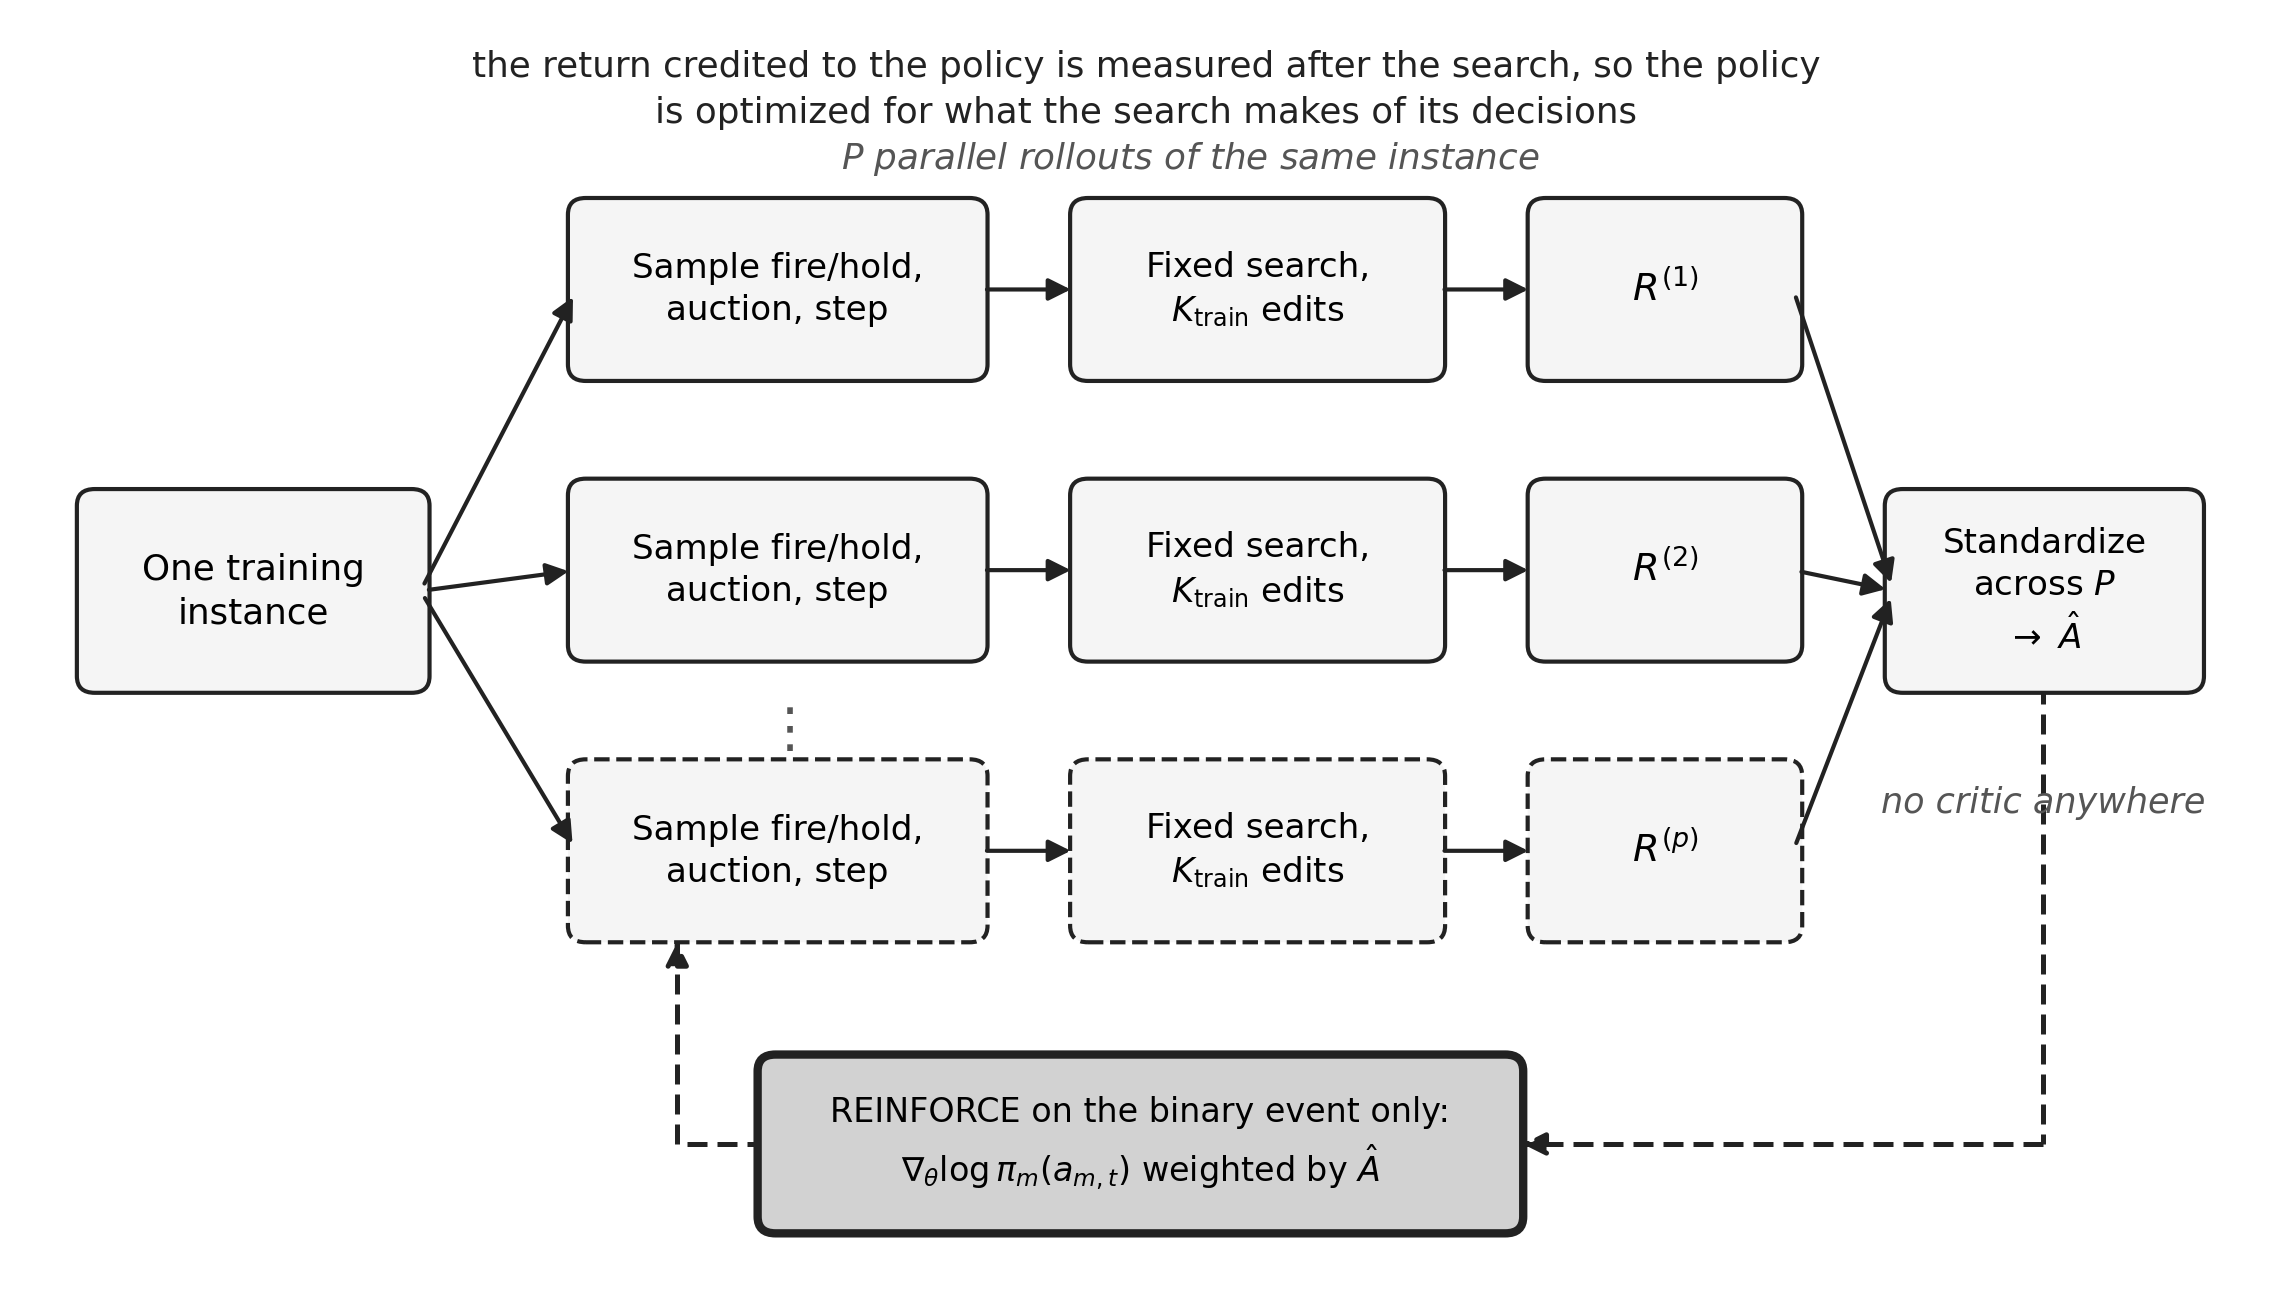
\includegraphics[width=\columnwidth]{figure/Training.png}
  \caption{Training. $P$ rollouts of one instance are sampled, each is passed
  through the fixed local search at a budget $K_{\mathrm{train}}$, and the
  post-search returns are standardized against one another to form the
  advantage. The gradient credits only the binary fire-or-hold event, not the
  target the assignment step chose. No value network appears at any point.}
  \label{fig:training}
\end{figure}

Two properties of this scheme are worth stating. First, the policy is
optimized for what the downstream machinery makes of its decisions rather than
for its own unsearched output, which is the relevant objective at deployment.
Second, because the search is fixed rather than learned, there is only one
moving target during training: the policy adapts to a stationary improvement
operator, rather than two networks each chasing the other's drift. The cost is
that the search absorbs some of the policy's mistakes before the objective is
measured, which attenuates the learning signal about exactly those mistakes;
Section~\ref{sec:limits} returns to this.
